\documentclass[a1paper,landscape,25pt]{tikzposter}

\usepackage{amsmath}
\usepackage{amssymb}
\usepackage{tikz}
\usetikzlibrary{calc}

\newcommand{\tikzmark}[2]{\tikz[baseline,anchor=base,remember picture] \node (#1) {#2};}

\usepackage{graphicx}
\usepackage{calc}
\newlength{\depthofsumsign}
\setlength{\depthofsumsign}{\depthof{$\sum$}}
\newlength{\totalheightofsumsign}
\newlength{\heightanddepthofargument}

\newcommand{\nsum}[1][1.4]{% only for \displaystyle
    \mathop{%
        \raisebox
            {-#1\depthofsumsign+1\depthofsumsign}
            {\scalebox
                {#1}
                {$\displaystyle\sum$}%
            }
    }
}
\newcommand{\resum}[1]{%
    \def\s{#1}
    \mathop{
        \mathpalette\resumaux{#1}
    }
}

\newcommand{\resumaux}[2]{% internally
    \sbox0{$#1#2$}
    \sbox1{$#1\sum$}
    \setlength{\heightanddepthofargument}{\wd0+\dp0}
    \setlength{\totalheightofsumsign}{\wd1+\dp1}
    \def\quot{\DivideLengths{\heightanddepthofargument}{\totalheightofsumsign}}
    \nsum[\quot]%
}

% http://tex.stackexchange.com/a/6424/16595
\makeatletter
\newcommand*{\DivideLengths}[2]{%
  \strip@pt\dimexpr\number\numexpr\number\dimexpr#1\relax*65536/\number\dimexpr#2\relax\relax sp\relax
}
\makeatother

\settitle{
  \vspace{-5cm}
  \centering \vbox{
\@titlegraphic \\[\TP@titlegraphictotitledistance] \centering
\color{titlefgcolor} {\bfseries \fontsize{90}{100} \sc \@title \par}
\vspace{2em}
}}

\title{Afgeleiden}

\addtolength{\jot}{1em}

\usetheme{Basic}
\usecolorstyle[colorPalette=BlueGrayOrange]{Britain}

\tikzposterlatexaffectionproofoff

\begin{document}

\maketitle

\begin{columns}
  \column{0.6}

  \block{Basisregels}{
    \LARGE
    \begin{align*}
      (c)' &= 0\\
      (x^n)' &= n x^{n-1}\qquad (n\in\mathbb{R})\\
      \big(c \cdot f(x)\big)' &= c \cdot f'(x)\\
      \big(f(x) \pm g(x)\big)' &= f'(x) \pm g'(x)
    \end{align*}
  }

  \block{Tabel met veelgebruikte afgeleiden}{
    \LARGE
    \begin{align*}
      (e^x)' &= e^x &
      (a^x)' &= a^x\ln(a) \ (a>0,\ a\neq 1)\\
      (\ln x)' &= \frac{1}{x}\ (x>0) &
      (\log_a x)' &= \frac{1}{x\ln(a)}\\
      (\sin x)' &= \cos x &
      (\cos x)' &= -\sin x\\
      (\tan x)' &= \frac{1}{\cos^2 x} &
      (\cot x)' &= -\frac{1}{\sin^2 x}\\
      (\sqrt{x})' &= \frac{1}{2\sqrt{x}}\ (x>0) &
      \left(\frac{1}{x}\right)' &= -\frac{1}{x^2}\ (x \neq 0)\\
      (\arcsin x)' &= \frac{1}{\sqrt{1-x^2}} &
      (\arccos x)' &= -\frac{1}{\sqrt{1-x^2}}\\
      (\arctan x)' &= \frac{1}{1+x^2} &
      (\text{arccot } x)' &= -\frac{1}{1+x^2}
    \end{align*}
  }

  \column{0.4}

  \block{Product, quotiënt, ketting}{
    \LARGE
    \begin{align*}
      (fg)' &= f'g + fg'\\[0.3em]
      \left(\frac{f}{g}\right)' &= \frac{f'g - fg'}{g^2}\qquad (g\neq 0)\\[0.3em]
      (f \circ g)'(x) &= f'\big(g(x)\big)\cdot g'(x)
    \end{align*}
  }

  \block{Definitie}{
    \LARGE
    \begin{align*}
      f'(x) &= \lim_{h \to 0} \frac{f(x+h) - f(x)}{h} \\[0.5em]
      f'(a) &= \lim_{x \to a} \frac{f(x) - f(a)}{x - a}
    \end{align*}
    \Large
    \begin{center}
    \end{center}
  }

  \block{Afgeleide is rico van de raaklijn}{
    \begin{center}
      \LARGE
      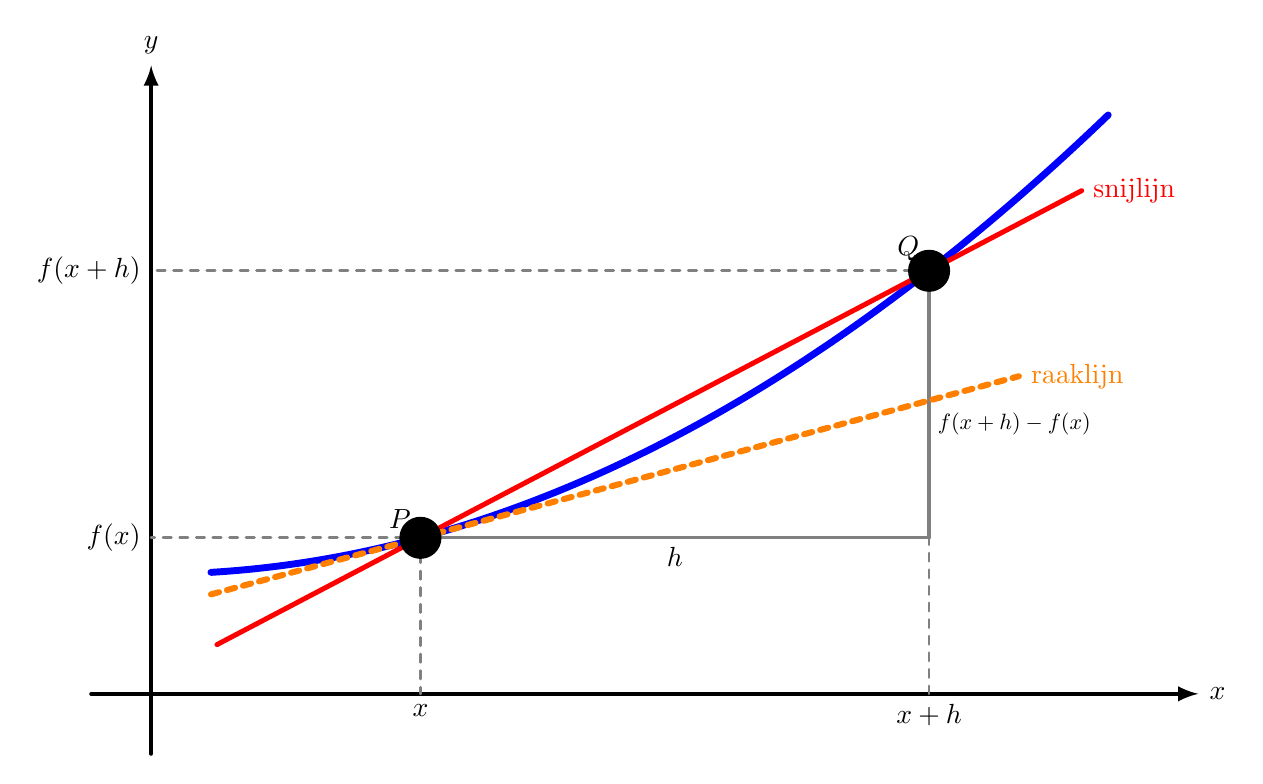
\begin{tikzpicture}[scale=3.8, line cap=round, line join=round, >=latex]
        % Definieer de functie y = 0.15x^2 + 0.4
        \def\fA{0.15} \def\fB{0.4}
        \pgfmathsetmacro{\xA}{0.9}
        \pgfmathsetmacro{\xB}{2.6}
        \pgfmathsetmacro{\yA}{\fA*\xA*\xA + \fB}
        \pgfmathsetmacro{\yB}{\fA*\xB*\xB + \fB}
        \pgfmathsetmacro{\slope}{2*\fA*\xA} % Rico van raaklijn: 2 * 0.15 * xA

        % Assen
        \draw[->, line width=1.5pt] (-0.2,0) -- (3.5,0) node[right] {$x$};
        \draw[->, line width=1.5pt] (0,-0.2) -- (0,2.1) node[above] {$y$};

        % De grafiek (blauw)
        \draw[line width=2.5pt, color=blue, samples=100, domain=0.2:3.2] plot (\x, {\fA*\x*\x + \fB});

        % Punten definities
        \coordinate (P) at (\xA,\yA);
        \coordinate (Q) at (\xB,\yB);
        \coordinate (R) at (\xB,\yA);

        % Projectielijnen naar de assen
        \draw[dashed, gray, line width=1pt] (\xA, \yA) -- (\xA, 0) node[below, black] {$x$};
        \draw[dashed, gray, line width=1pt] (\xB, \yB) -- (\xB, 0) node[below, black] {$x+h$};
        \draw[dashed, gray, line width=1pt] (\xA, \yA) -- (0, \yA) node[left, black] {$f(x)$};
        \draw[dashed, gray, line width=1pt] (\xB, \yB) -- (0, \yB) node[left, black] {$f(x+h)$};

        % Hellingsdriehoek (grijs)
        \draw[line width=1.2pt, gray] (P) -- (R) node[midway, inner sep=1pt, below, black, yshift=-2pt] {$h$};
        \draw[line width=1.2pt, gray] (R) -- (Q) node[midway, below right, black, scale=0.8] {$f(x+h)-f(x)$};

        % Snijlijn/Secant (rood)
        \draw[line width=1.8pt, color=red] ($ (P)!-0.4!(Q) $) -- ($ (P)!1.3!(Q) $) node[right] {snijlijn};

        % Raaklijn (oranje, gestippeld)
        \draw[line width=2.2pt, color=orange, dashed] (\xA-0.7, {\yA - \slope*0.7}) -- (\xA+2, {\yA + \slope*2.0}) node[right] {raaklijn};

        % Punten zelf
        \fill[black] (P) circle (2pt) node[above left] {$P$};
        \fill[black] (Q) circle (2pt) node[above left] {$Q$};

        % Conceptuele tekst onderaan
%        \node[anchor=north] at (1.75, -0.6) {\large Wanneer $h \to 0$, nadert de snijlijn de raaklijn.};
      \end{tikzpicture}
    \end{center}
  }

\end{columns}

\end{document}
